\documentclass[compress]{beamer}

\usetheme{onera}
\usepackage{listings,algorithm,algorithmic}

\title[SEM GI313 - Planification]{{\Large Planification}\\GI313 - Optimisation}
\author[Charles Lesire]{Charles Lesire-Cabaniols (ONERA / DCSD)}
\date[2010-2011]{3A-SEM - 2010-2011}

\graphicspath{{./},{figures/}}
\lstset{basicstyle=\tiny,tabsize=2,%frame=single,%
	emph={define,domain,requirements,strips,typing,types,predicates,
		action,parameters,precondition,vars,effect,objects,init,goal},%
	emphstyle=\bf}

\begin{document}
\begin{frame}
\tableofcontents[hidesubsections]
\end{frame}

%%%%% INTRODUCTION %%%%%
\section{Introduction}
\begin{frame}
\tableofcontents[hideothersubsections]
\end{frame}

\subsection{Problèmes de planification}
\begin{frame}{Qu'est-ce que planifier ?}
\begin{itemize}
\item \structure{Planning :} Analyse, vérification d'un plan
	\begin{itemize}
	\item on connaît les actions, leur organisation, leurs ressources
	\item on vérifie les contraintes, on obtient les chemins critiques
	\item[ex:] élaboration interactive de plans, réseaux PERT\dots
	\end{itemize}
\end{itemize}
\begin{tikzpicture}[scale=.6,transform shape,%
	circle/.style={circle split, draw=black, thick,%
		inner sep=0pt, node distance=3cm}]
\draw[use as bounding box, transparent] (0,-3) grid[help lines] (15,4);
\path[overlay]<2> node[circle] (n0) {0 \nodepart{lower} $\begin{array}{l|r}0&0\end{array}$};
\path[overlay]<3-> node[circle,draw=red] (n0) {%
	\color{red}0 \nodepart{lower} $\begin{array}{l|r}0&0\end{array}$};
\foreach \n/\e/\l/\pos/\rel/\red in {%
	1/30/30/right of/0/1,
	2/120/120/right of/1/1,
	4/40/200/below of/2/0,
	6/150/150/right of/2/1,
	3/150/210/above of/6/0,
	5/50/210/below of/6/0,
	7/210/210/right of/6/1,
	8/220/220/right of/7/1%
	} {%
\ifthenelse{\equal{\red}{1}}{% Le noeud est dans le chemin critique
	\path[overlay]<2> node[circle,\pos=n\rel] (n\n) {%
		\n \nodepart{lower} $\begin{array}{l|r}\e&\l\end{array}$};
	\path[overlay]<3-> node[circle,,\pos=n\rel,draw=red] (n\n) {%
		\color{red}\n \nodepart{lower} $\begin{array}{l|r}\e&\l\end{array}$};
}{% sinon
	\path[overlay]<2-> node[circle,\pos=n\rel] (n\n) {%
		\n \nodepart{lower} $\begin{array}{l|r}\e&\l\end{array}$};	
}}
\foreach \a/\b/\red in {0/1, 1/2, 1/4, 2/3, 2/6, 4/5, 3/7, 6/7, 5/7, 7/8} {%
\ifthenelse{\equal{\red}{1}}{% Le noeud est dans le chemin critique
	\path[overlay,draw]<2> (n\a) edge[->] (n\b);
	\path[overlay,draw=red]<3-> (n\a) edge[->] (n\b);
}{% sinon
	\path[overlay,draw]<2-> (n\a) edge[->] (n\b);
}}
\end{tikzpicture}
\end{frame}

\begin{frame}{Qu'est-ce que planifier ?}
\begin{itemize}
\item \structure{Ordonnancement :} Organisation d'un plan
	\begin{itemize}
	\item on connaît les actions à faire
	\item on cherche leur organisation, les ressources à allouer
	\item[ex:] ordonnancement, gestion de ressources\dots
	\end{itemize}
\end{itemize}
\begin{center}
\visible<2->{%
	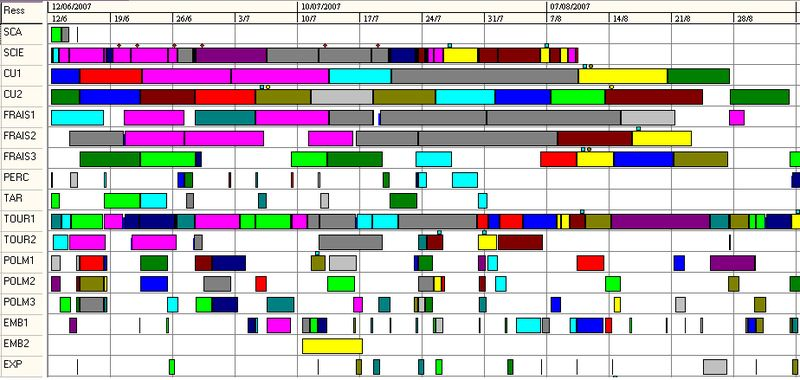
\includegraphics[width=.8\linewidth]{ordonnancement}%
}
\end{center}
\end{frame}

\begin{frame}{Qu'est-ce que planifier ?}
\begin{itemize}
\item \structure{Planification :} Synthèse d'un plan
	\begin{itemize}
	\item on connaît les buts à satisfaire, les actions possibles
	\item on cherche leur les actions à faire pour atteindre ces buts, 
		leur organisation, les ressources à allouer
	\item[ex:] gestion de l'activité d'un système autonome\dots
	\end{itemize}
\end{itemize}
\end{frame}

\begin{frame}{Problèmes de planification}
\begin{itemize}
\item Ingrédients :
	\begin{itemize}
	\item Modèle de l'environnement
	\item Modèles des actions possibles
	\item Spécification des objectifs (buts, critères)
	\item Données sensorielles sur l'état initial et l'état courant (si utilisation en ligne)
	\end{itemize}
\item Diverses formes selon :
	\begin{itemize}
	\item Le type de tâches à planifier
	\item La nature des modèles
	\end{itemize}
\end{itemize}
\end{frame}

\subsection{Modèles de planification}
\begin{frame}{Modèle de la planification}
Système Etat-Transition $\Sigma = (S, A, E, \gamma)$
\begin{itemize}
\item[$S$] ensemble dénombrable d'\structure{états}
\item[$A$] ensemble fini de symboles d'\structure{actions}
\item[$E$] ensemble fini de symboles d'\structure{événements}
\item[$\gamma$] fonction de transition d'états
	$$\gamma: S \times (A \cup E) \rightarrow 2^S$$
	\begin{itemize}
	\item si $u \in E$, $\gamma(s, u)$ transitions \structure{contingentes}
	\item si $u \in A$, $\gamma(s, u)$ transitions \structure{contrôlées}
	\end{itemize}
\end{itemize}
\begin{block}{Problème de planification}
quelles \structure{actions} appliquer à quels états en vue de réaliser des \structure{objectifs} ?
\end{block}
\end{frame}

\begin{frame}{Modèle de la planification}
\begin{center}
\begin{tikzpicture}[%
	block/.style={draw,fill=blue!20,rectangle,minimum height=3em,minimum width=6em},%
	pin edge={to-,thin,black},
	auto, node distance=2cm, >=latex']
\node[block,pin={left:But, Etat initial},pin={above:Description de $\Sigma$}] (planif) {Planificateur};
\node[block,below of=planif] (control) {Contrôleur};
\node[block,below of=control,pin={below:Evénements}] (system) {Système $\Sigma$};
\draw[->] (planif) -- node{Plan} (control);
\draw[->] (control.east) -- +(1,0) |- node{Actions} (system.east);
\draw[->] (system.west) -- +(-1,0) |- node{\alt<2>{\structure{Observations}}{Etat}} (control.west);
\end{tikzpicture}
\end{center}
\end{frame}

\begin{frame}{Modèle de la planification}
\begin{itemize}[<+->]
\item Plan : $$\pi: S' \subset S \rightarrow A$$
\item Observations :
	\begin{itemize}
	\item $O$ ensemble fini d'\structure{observations}
	\item Fonction d'observation $\eta: S \rightarrow O$
	\end{itemize}
\item Plan : $$\pi: O' \subset O \rightarrow A$$
\end{itemize}
\end{frame}

\begin{frame}{Modèle de la planification}
\begin{itemize}
\item<+-> Hypothèses classiques :
	\begin{enumerate}
	\item $\Sigma$ fini (monde fermé)
	\item $\Sigma$ observable ($\eta = I$)
	\item $\Sigma$ déterministe ($|\gamma(s,u) \leq 1$)
	\item $\Sigma$ statique
	\item Buts = états explicites
	\item Temps implicite
	\item Traitement hors-ligne
	\end{enumerate}
\item<+-> $2+3 \Rightarrow$ contrôle en boucle ouverte
\end{itemize}
\end{frame}

\begin{frame}{Formes de planification}
\begin{itemize}
\item Planification de mouvements
	\begin{itemize}
	\item Trajectoires géométriques en 3D, lois de commande le long des trajectoires
	\end{itemize}
\item Planification de la perception
	\begin{itemize}
	\item Quelle information est requise ?
	\item Quand ? Où ? Comment ? Pour quoi ?
	\end{itemize}
\item Planification de tâches de manipulation
	\begin{itemize}
	\item Primitives sensori-motrices, utilisant les forces, la vision\dots
	\end{itemize}
\end{itemize}
\end{frame}

\begin{frame}{Formes de planification}
\begin{itemize}
\item Planification de la communication
	\begin{itemize}
	\item Interaction homme-robot
	\item Coopération multi-robots
	\item Quelles requêtes, comment, quels retours ?
	\end{itemize}
\item Planification de tâches générique
	\begin{itemize}
	\item Modèles et algorithmes généraux à plusieurs types de problèmes
	\end{itemize}
\end{itemize}
\end{frame}

%%%%% REPRESENTATION %%%%%
\section{Représentations}
\begin{frame}
\tableofcontents[hideothersubsections]
\end{frame}

\subsection{Planification de tâches}
\begin{frame}{Planification de tâches}
\begin{itemize}
\item Définition :
	\begin{itemize}
	\item Synthèse d'une trajectoire abstraite dans un \structure{espace de recherche}
	\item pur choisir et organiser des actions en \structure{prédisant} leurs effets
	\item en vue de \structure{satisfaire un but} ou un critère
	\end{itemize}
\item Ingrédients :
	\begin{itemize}
	\item Description des états du monde et des buts
	\item Description des actions
	\end{itemize}
\end{itemize}
\end{frame}

\begin{frame}{Planification de tâches}
\begin{itemize}
\item Système Etat-Transition $\Sigma = (S,A,\gamma)$
	\begin{itemize}
	\item[$S$] ensemble fini d'\structure{états}
	\item[$A$] ensemble fini de symboles d'\structure{actions}
	\item[$\gamma$] fonction de transition d'états
		$$\gamma: S \times A \rightarrow A$$
	\end{itemize}
\end{itemize}
\end{frame}

\subsection{Représentation graphique}
\begin{frame}{Représentation graphique}
\begin{itemize}
\item Exemple des robots-dockers
	\begin{itemize}
	\item $N$ sites
	\item $K$ conteneurs à déplacer entre ces sites
	\item $P$ piles réparties sur ces sites
	\item $R$ robots pouvant acheminer ces conteneurs
	\end{itemize}
\item Actions :
	\begin{itemize}
	\item \structure{move} un robot $r$ se déplace de $l$ à $l'$
	\item \structure{load} un robot $r$ charge un conteneur $k$ porté par un bras $c$
	\item \structure{unload}
	\item \structure{take} un bras $c$ saisit un conteneur $k$ sur le sommet d'une pile $p$
	\item \structure{put}
	\end{itemize}
\end{itemize}
\end{frame}

\begin{frame}{Représentation graphique}
\begin{itemize}
\item Complexité
	\begin{itemize}
	\item Nombre d'états possibles : $\mathcal{O}(n^r \, p^k \, k!)$
	\item $n = 5$, $p = 15$, $r = 3$, $k = 100 \Rightarrow \sim 10^{277}$ états !!
	\end{itemize}
\item Impossible de construire $\Sigma$ explicitement
	(et donc d'appliquer des techniques de recherche de chemin dans des graphes)
\end{itemize}
\end{frame}

\subsection{Langage de représentation}
\begin{frame}{Langage de représentation}
\begin{itemize}
\item Langage de représentation des états et des actions
\item Hypothèses classiques :
	\begin{itemize}
	\item transitions instantannées, pas de durée, pas de parallélisme
	\item monde statique, pas de transitions contingentes
	\item connaissance complète
	\item actions déterministes
	\end{itemize}
\item Formule : conjonction de littéraux
\item Hypothèse du monde clos : ce qui n'est pas explicitement affirmé est faux
\end{itemize}
\end{frame}

\begin{frame}[containsverbatim]{Langage de représentation}
\begin{lstlisting}
(define (domain dock-worker-robot)
	(:requirements :strips :typing)
	(:types
		location ; several connected locations
		pile ; attached to location holds a pallet and a stack of containers
		robot ; holds at most 1 container, only 1 robot per location
		crane ; belongs to a location to pickup containres
		container
	)
	(:predicates
		(adjacent ?l1 ?l2 - location) ; l1 is adjacent to l2
		(attached ?p - pile ?l - location) ; p attached to l
		(belong ?c - crane ?l - location) ; c belongs to l
		(at ?r - robot ?l - location) ; r is at l
		(occupied ?l - location) ; there is a robot at l
		(loaded ?r - robot ?k - container) ; r loaded with container k
		(unloaded ?r - robot) ; r is empty
		(holding ?c - crane ?k - container) ; c is holding k
		(empty ?c - crane) ; c is empty
		(in ?k - container ?p - pile) ; k is within p
		(top ?k - container ?p - pile) ; k is on top of p
		(on ?k1 ?k2 - container) ; k1 is on k2
	)
\end{lstlisting}
\end{frame}

\begin{frame}[containsverbatim]{Langage de représentation}
\begin{lstlisting}
(:action move
	:parameters (?r - robot ?from ?to - location)
	:precondition (and (adjacent ?from ?to) (at ?r ?from) (not (occupied ?to)))
	: effect (and (at ?r ?to) (not (occupied ?from)) (occupied ?to)
		(not (at ?r ?from))))
(: action load
	:parameters (?c - crane ?k - container ?r - robot)
	:vars (?l - location)
	:precondition (and (at ?r ?l) (belong ?c ?l) (holding ?c ?k) (unloaded ?r))
	:effect (and (loaded ?r ?k) (not (unloaded ?r)) (empty ?c)
		(not (holding ?c ?k))))
(: action unload
	:parameters (?c - crane ?k - container ?r - robot)
	:vars (?l - location)
	:precondition (and (at ?r ?l) (belong ?c ?l) (loaded ?r ?k) (empty ?c))
	:effect (and (unloaded ?r) (holding ?c ?k) (not (loaded ?r ?k))
		(not (empty ?c))))
(: action take
	:parameters (?c - crane ?k - container ?p - pile)
	:vars (?l - location ?else container)
	:precondition (and (belong ?c ?l) (attached ?p ?l) (empty ?c)
		(in ?k ?p) (top ?k ?p) (on ?k ?else))
	:effect (and (holding ?c ?k) (top ?else ?p) (not (in ?k ?p))
		(not (top ?k ?p)) (not (on ?k ?else)) (not (empty ?c))))
(: action put
	:parameters (?c - crane ?k - container ?p - pile)
	:vars (?l - location ?else container)
	:precondition (and (belong ?c ?l) (attached ?p ?l)
		(holding ?c ?k) (top ?else ?p))
	:effect (and (in ?k ?p) (top ?k ?p) (on ?k ?else)
		(not (top ?else ?p)) (not (holding ?c ?k)) (empty ?c)))
\end{lstlisting}
\end{frame}

\begin{frame}[containsverbatim]{Langage de représentation}
\begin{lstlisting}
(define (problem dwrpb1)
	(:domain dock-worker-robot)
	(:objects
		r - robot
		l1 l2 - location
		c1 c2 - crane
		p1 q1 p2 q2 - pile
		a b c d e f pallet - container)
	(:init
		(adjacent l1 l2) (adjacent l2 l1)
		(attached p1 l1) (attached q1 l1) (attached p2 l2) (attached q2 l2)
		(belong c1 l1) (belong c2 l2)
		(in a p1) (in b p1) (in c p1)
		(in d q1) (in e q1) (in f q1)
		(on a pallet) (on b a) (on c b)
		(on d pallet) (on e d) (on f e)
		(top c p1) (top f q1) (top pallet p2) (top pallet q2)
		(at r l1) (unloaded r) (occupied l1)
		(empty c1) (empty c2))
	(:goal
		(and (in a p2) (in b p2) (in c p2)
			(in d q2) (in e q2) (in f q2))))
\end{lstlisting}
\end{frame}

\begin{frame}{Langage de représentation}
\begin{itemize}
\item \structure{forall (?x - type)} : boucle sur les éléments d'un type
\item \structure{when cond effect} : applique l'effet lorsque la condition est vraie
\end{itemize}
\end{frame}

%%%%% PLANIFICATION %%%%%
\section{Planification dans l'espace d'état}
\begin{frame}
\tableofcontents[hideothersubsections]
\end{frame}

\subsection{Espace d'état}
\begin{frame}{Transitions}
\begin{itemize}
\item Calcul progressif : \structure{result(a, s)}
	$$ s \models precond(a) \Rightarrow s' = (s - effets^-(a)) \cup effets^+(a)$$
\item Calcul inverse : \structure{regress($\gamma$, a)}
	$$ \gamma \cap effets^-(a) = \emptyset \Rightarrow regress = precond(a) \cup (\gamma - effets^+(a))$$
\end{itemize}
\end{frame}

\subsection{Recherche en avant}
\begin{frame}{Forward}
\begin{block}{$Forward(S, S_g, path)$}
	\begin{algorithmic}
	\IF {$s \models S_g$ }
		\RETURN path
	\ELSE
		\STATE applicables $\leftarrow \{ a \in A \, / \, s \models precond(a) \}$
		\IF {applicables $= \emptyset$}
			\RETURN FAIL
		\ELSE
			\STATE \structure{Choose} $a \in$ applicables
			\RETURN $Forward(result(a, s), S_g, path.a)$
		\ENDIF
	\ENDIF
	\end{algorithmic}
\end{block}
\end{frame}

\begin{frame}{Forward}
\begin{itemize}
\item $Forward(s_0, S_g, \emptyset)$
\item Algorithme simple
\item Algorithme complet
\item Méthode \structure{Choose} permet de guider la recherche :
	\begin{itemize}
	\item en largeur (Breath-First Search)
	\item en profondeur (Depth-First Search)
	\item en prenant en compte le coût des actions (Best-First Search)
	\item guidée par une heuristique
	\end{itemize}
\end{itemize}
\end{frame}

\begin{frame}{$A^*$}
\begin{algorithmic}
\REQUIRE $G=(S,E)$ le graphe implicite, $s_0$ état initial, $S_g$ but
\STATE $\forall s \in S, \, g(s) \leftarrow \infty, p(s) \leftarrow s \qquad
	c(s_0) \leftarrow 0$, $\mathcal{O} \leftarrow \{s_0\}$
\WHILE {$\mathcal{O} \neq \emptyset$}
	\STATE $x \leftarrow argmax_{argmin \, g(i) + h(i)} \, g(i)$
    \IF {$x \models S_g$}
    	\RETURN SUCCESS
    \ENDIF
	\STATE $\mathcal{O} \leftarrow \mathcal{O} / \{x\}$
	\FORALL {$y \in S \, / \, (x,y) \in E$}
		\IF {$g(y) > g(x) + k(x,y)$}
			\STATE $g(y) \leftarrow g(x) + k(x,y)$
			\STATE $p(y) \leftarrow x$
			\STATE $\mathcal{O} \leftarrow \mathcal{O} \cup \{y\}$
		\ENDIF
	\ENDFOR
\ENDWHILE
\end{algorithmic}
\end{frame}

\begin{frame}{$A^*$}
\begin{itemize}
\item Si $G$ est fini, l'algorithme \structure{termine}
\item Si $h$ est minorante, l'algorithme est \structure{complet} et \structure{optimal}
$$h \mbox{ minorante} \Leftrightarrow \forall s \in S, \; h(s) \leq g(s)$$
\item Complexité :
	\begin{itemize}
	\item $h$ minorante : $\mathcal{O}(N^2)$
	\item $h$ monotone : $\mathcal{O}(N)$
	\end{itemize}
$$h \mbox{ monotone} \Leftrightarrow \forall (u, v) \in E, \; h(u) - h(v) \leq k(u,v)$$
\end{itemize}
\end{frame}

\begin{frame}{$A^*$}
\begin{center}
	\begin{tikzpicture}[scale=.7, transform shape]
	\node[state] (B) at (3,6) {};
	\node[state] (D) at (9,6) {};
	\node[state] (F) at (3,3) {};
	\node[state] (G) at (6,3) {};
	\node[state] (H) at (9,3) {};
	\node[state] (I) at (0,0) {};
	\node[state, fill=red!30] (J) at (3,0) {0};
	\node[state] (K) at (6,0) {};
	\draw[->, thick] (B) edge node {4} (D)
					(F) edge node {2} (B) edge node {8} (D)
					(G) edge node {2} (H)
					(H) edge node {1} (D)
					(I) edge node {6} (B) edge node {1} (F)
					(J) edge node {5} (I) edge node {7} (G) edge node {6} (K)
					(K) edge node {2} (G) edge node {1} (H);
	\end{tikzpicture}
\end{center}
\end{frame}

\subsection{Heuristiques}
\begin{frame}{Heuristiques}
\begin{itemize}
\item \structure{Relaxation} : on simplifie le problème pour estimer les coûts
\item Compromis entre temps de calcul et qualité de l'heuristique
\item Voyageur de commerce :
	\begin{itemize}
	\item $h_1 = d(r,s)$ : distance à la ville suivante
	\item $h_2 = d(r,s) + \Sigma_i \min_x d(x, s_i)$ : on minimise les distances aux villes restantes
	\item $h_3 = d(r,s) + $ coût d'un arbre de recouvrement minimal
	\end{itemize}
\end{itemize}
\end{frame}

\begin{frame}{Heuristiques}
\begin{block}{Relaxation}
	\begin{itemize}
	\item Ne prendre en compte que les $effets^+$
		\begin{itemize}
		\item admissible, mais difficile à calculer
		\end{itemize}
	\item Supporser l'indépendance des sous-buts
	\end{itemize}
\end{block}
\end{frame}

\begin{frame}{Heuristiques}
\begin{block}{Relaxation}
	\begin{itemize}
	\item Coût pour réaliser $p$ à partir de $s$ :
	$$h(p,s) = \left\{\begin{array}{ll}
		O & \mbox{si } s \models p\\
		\min_a (1 + h(precond(a), s)) & \mbox{sinon}
		\end{array}\right.$$
	\item Heuristiques possibles :
		\begin{itemize}
		\item Somme des coûts des litéraux
		$$h(s) = \Sigma_{p \in S_g} h(p,s)$$
		\item Litéral le plus coûteux
		$$h(s) = \max_{p \in S_g} h(p,s)$$
		\end{itemize}
	\end{itemize}
\end{block}
\end{frame}

\subsection{Recherche en arrière}
\begin{frame}{Backward}
\begin{block}{$Backward(s_0, \gamma, path)$}
	\begin{algorithmic}
	\IF {$s_0 \models \gamma$ }
		\RETURN path
	\ELSE
		\STATE \structure{Choose} $g \in \gamma$
		\STATE relevant $\leftarrow \{a \in A \, / \, effts(a) \models g\}$
		\IF {relevant $= \emptyset$}
			\RETURN FAIL
		\ELSE
			\STATE \structure{Choose} $a \in$ relevant
			\RETURN $Forward(s_0, regress(\gamma, a), a.path)$
		\ENDIF
	\ENDIF
	\end{algorithmic}
\end{block}
\end{frame}

%%%%% FURTHER %%%%%
\section{Allez plus loin en planification}
\begin{frame}
\tableofcontents[hideothersubsections]
\end{frame}

\subsection{Planification dans l'espace des plans}
\begin{frame}{Planification dans l'espace des plans}
\begin{itemize}
\item L'espace de recherche n'est plus l'espace d'état mais l'espace des plans
\item L'algorithme passe d'un plan à un autre en essayant de l'améliorer
\item Au départ, seulement l'état initial et les buts sont dans le plan
\item Le principe est de résoudre les \structure{défauts} du plan en insérant des actions
\item Moindre engagement (pas d'action inutile)
\item PSP, POP
\end{itemize}
\end{frame}

\subsection{Planification disjonctive}
\begin{frame}{Planification disjonctive}
\begin{itemize}
\item Disjonction pas gérable par les méthodes précédentes
	\begin{itemize}
	\item traitent un état/un but après l'autre
	\end{itemize}
\item \structure{GraphPlan}
	\begin{itemize}
	\item Accessibilité des litéraux buts
	\item Phase de \structure{construction} : élaboration descendante d'un P-graphe
	\item Phase d'\structure{extraction} : recherche ascendant à partir des buts
	\end{itemize}
\end{itemize}
\end{frame}

\subsection{Planification hiérarchique}
\begin{frame}{Planification hiérarchique}
\begin{itemize}
\item Structuration hiérarchique des actions
\item Fournit une heuristique pour la recherche
\item PSP, HTN, UMCP
\end{itemize}
\begin{center}
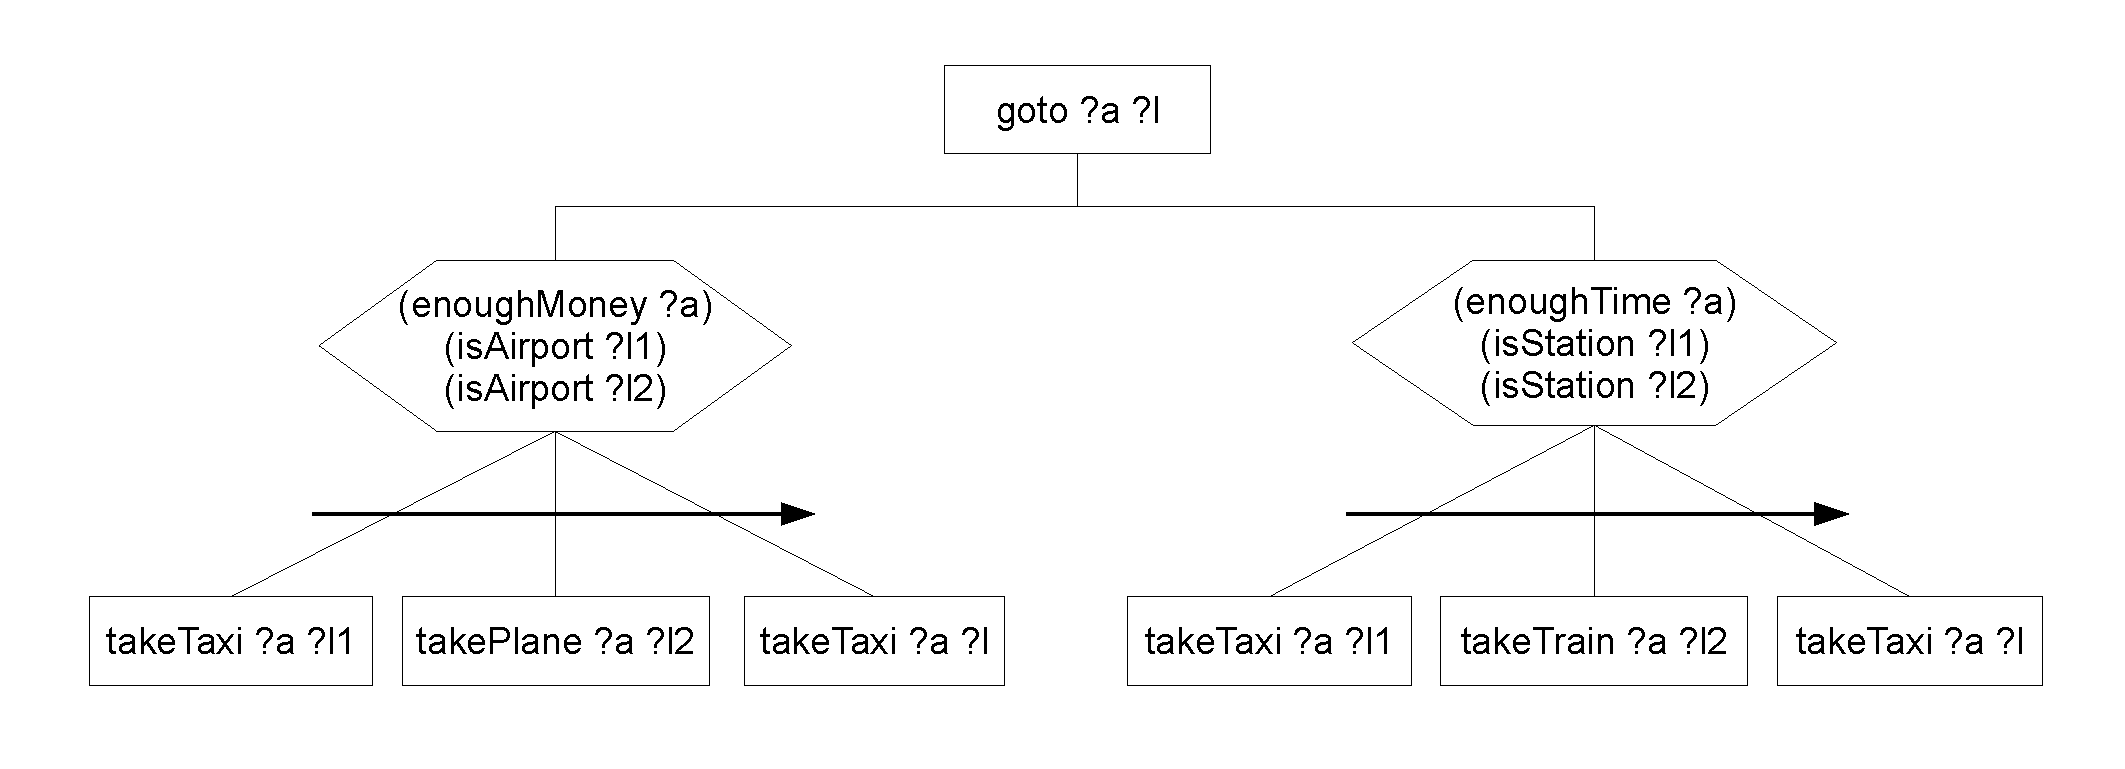
\includegraphics[width=.6\linewidth]{exHTN}
\end{center}
\end{frame}

\subsection{Représentation du temps}
\begin{frame}{Traitement du temps}
\begin{itemize}
\item Le temps est une ressource particulière
	\begin{itemize}
	\item écoulement indépendant de l'action
	\item disponible pour tous (parallélisme)
	\end{itemize}
\item Le temps est structuré par une relation transitive et asymétrique
	\begin{itemize}
	\item il est irréversible
	\item il ordonne la causalité
	\end{itemize}
\end{itemize}
\end{frame}

\begin{frame}{Représentation du temps}
\begin{itemize}
\item Représentation géométrique
\item Représentation logique
	\begin{itemize}
	\item argument d'un prédicat, en spécifiant les changements d'état
	\item prédicats spécifiques pour les relations temporelles (algèbre d'Allen)
	\item logiques temporisés (avec des valeurs numériques)
	\end{itemize}
\end{itemize}
\end{frame}

\begin{frame}{Planification temporelle}
\begin{itemize}
\item Programmation par contrainte avec des contraintes temporelles
\item Planification dans l'espace des plans, plans temporels
	\begin{itemize}
	\item IxTeT, RAX, parcPLAN
	\end{itemize}
\end{itemize}
\end{frame}

%%%%% BE %%%%%
\section{BE}
\begin{frame}
\tableofcontents[hideothersubsections]
\end{frame}

\subsection{Mission}
\begin{frame}{Mission}
\begin{itemize}
\item Mission de recherche et d'extinction d'incendie
\item Zone de missions découpée en sous-zones
\item Exploration des sous-zones à la recherche d'un feu
\item Extinction d'un feu si trouvé
\item Retour à la base si pas de feu ou plus de cartouche d'extinction
\end{itemize}
\end{frame}

\subsection{Sujet ARD}
\begin{frame}{Sujet Application Robotique Dronique}
\begin{itemize}
\item Développer l'architecture embarquée pour réaliser cette mission
\item Environnement de développement en C++ à base de composants
\item Composant de navigation (existants)
\item Composant de détection (blob rouge sur image / à développer)
\item Composant de cartographie (à développer)
\item Composant de supervision (à développer)
\end{itemize}
\end{frame}

\subsection{Sujet Planification}
\begin{frame}{Sujet de planification}
\begin{itemize}
\item Quelles actions réaliser pour accomplir la mission ?
\item Planification des actions, qui seront intégrées dans le superviseur
\item Algorithme FF (Fast Forward)
\end{itemize}
\begin{enumerate}
\item Modélisation le domaine de planification (prédicats, actions)
\item Modéliser un premier problème (en faisant des hypothèses sur l'environnement)
\item Générer un plan
\item Proposer une façon de rendre ce plan robuste aux défauts des hypothèses posées
\end{enumerate}
\end{frame}

\end{document}
